\documentclass[11pt,twoside,a4paper]{article}
\usepackage[dutch]{babel}
\usepackage{a4wide,times}
\usepackage{pdfpages}
\usepackage{graphicx}
\usepackage{float}
\usepackage{rotating}
\usepackage{listings}
\usepackage{hyperref}
\usepackage{enumitem}
\usepackage[utf8]{inputenc}
\usepackage{siunitx}
\usepackage{nameref}
\begin{document}

\begin{centering}
\title{\textbf{Reflectie op het plan van aanpak}}
\author{Projectgroep A1}
\date{\today}

\maketitle
\end{centering}

\section{Introductie}
Klopt de planning nog? Moeten er eventueel aanpassingen gedaan worden aan de manier van werken of de planning? Hieronder zijn een paar verbeteringen aan het plan van aanpak aangebracht en de planning is weer up-to-date.

\section{Projectopdracht en -activiteiten}
De projectopdracht is inmiddels verder uitgewerkt en verbeterd. Er wordt nu niet meer in duo's gewerkt, omdat bleek dat het alarm-blok relatief simpel bleek te zijn, waar dus niet constant twee man naar hoeven te kijken, en de LCD-controller bleek veel te veel voor twee personen.

\section{Planning}
De planning in het plan van aanpak was niet gedetailleerd genoeg, dus die is verder uitgewerkt.\\
Volgens de planning moet de ontwerpfase al voorbij zijn en zou er nu getest moeten worden. De meeste code is af, maar er is vertraging opgelopen bij het LCD-blok. De LCD-controller bestaat uit vijf modules en dit bleek te veel werk te zijn voor twee personen. In figuur \ref{fig:planning} is de planning verder uitgewerkt en bijgewerkt.

\begin{figure}[h!]
\center
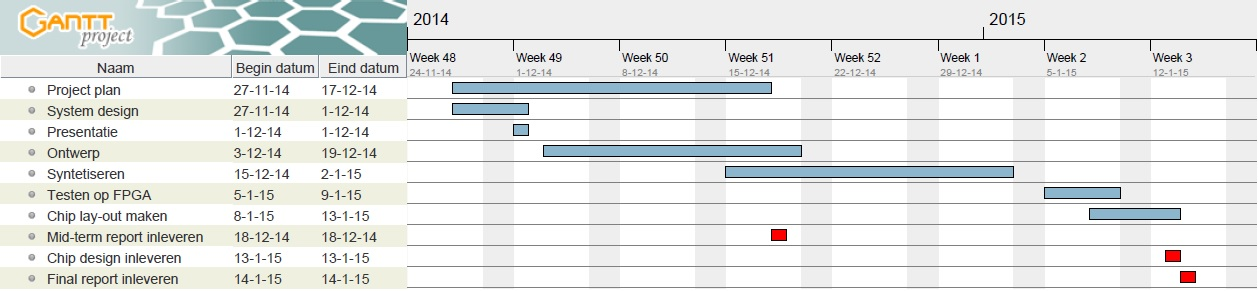
\includegraphics[width=15cm]{planning2}
\caption{Planning versie 2.0}
\label{fig:planning}
\end{figure}

\newpage
\section{Risico's}
Het grootste technische risico is dat het DCF signaal niet werkt. Om toch het systeem te kunnen testen terwijl de ontvangst van het signaal slecht is, is ons een VHDL code aangeboden om op een FPGA te kunnen zetten. Op die manier kan er wel getest worden of de rest van het systeem werkt zonder daadwerkelijk DCF signaal.\\
Een probleem wat zich nu ook voor gaat doen is de beschikbare plaats op de chip. Er moet steeds goed in het achterhoofd gehouden worden hoeveel plaats er is op de chip. Aangezien er een paar grote bitvectoren van het ene blok naar het andere moet, zal ook de bedrading een groot deel van de chip in beslag nemen. Daarom is al besloten om een microcontroller te maken tussen de chip en de LCD, waar de karakters in opgeslagen zijn.

\end{document}